\documentclass[12pt,letterpaper]{article}
\usepackage{fullpage}
\usepackage[top=2cm, bottom=4.5cm, left=2.5cm, right=2.5cm]{geometry}
\usepackage{amsmath,amsthm,amsfonts,amssymb,amscd}
\usepackage{lastpage}
\usepackage{enumerate}
\usepackage{subfigure}
\usepackage{fancyhdr}
\usepackage{mathrsfs}
\usepackage{xcolor}
\usepackage{graphicx}
\usepackage{listings}
\usepackage{hyperref}

\hypersetup{%
  colorlinks=true,
  linkcolor=blue,
  linkbordercolor={0 0 1}
}
 
\renewcommand\lstlistingname{Algorithm}
\renewcommand\lstlistlistingname{Algorithms}
\def\lstlistingautorefname{Alg.}

\lstdefinestyle{c++}{
    language        = c++,
    frame           = lines, 
    basicstyle      = \footnotesize,
    keywordstyle    = \color{blue},
    stringstyle     = \color{green},
    commentstyle    = \color{red}\ttfamily,
    breaklines = true
}

\setlength{\parindent}{0.0in}
\setlength{\parskip}{0.05in}

% Edit these as appropriate
\newcommand\course{Numerical Analysis}
\newcommand\hwnumber{2}                  % <-- homework number
\newcommand\NetIDa{3190103519 }           % <-- NetID of person #1
\newcommand\NetIDb{Li Yangye}           % <-- NetID of person #2 (Comment this line out for problem sets)

\pagestyle{fancyplain}
\headheight 35pt
\lhead{\NetIDa}
\lhead{\NetIDa\\\NetIDb}                 % <-- Comment this line out for problem sets (make sure you are person #1)
\chead{\textbf{\Large Homework \hwnumber}}
\rhead{\course \\ \today}
\lfoot{}
\cfoot{}
\rfoot{\small\thepage}
\headsep 1.5em

\begin{document}

\section*{Homework2 Program Report}


  \subsection*{} 
    Problem B: test Newton Formula on $\frac{1}{1+x^2}$.\\
    n = 2: $1-0.0384615x^{2}$\\
    n = 4: $1-0.171088x^{2}+0.00530504x^{4}$\\
    n = 6: $1-0.351364x^{2}+0.0335319x^{4}-0.000840633x^{6}$\\
    n = 8: $1-0.528121x^{2}+0.0981875x^{4}-0.00658016x^{6}+0.000137445x^{8}$\\
    \begin{figure}[h]
      \centering
      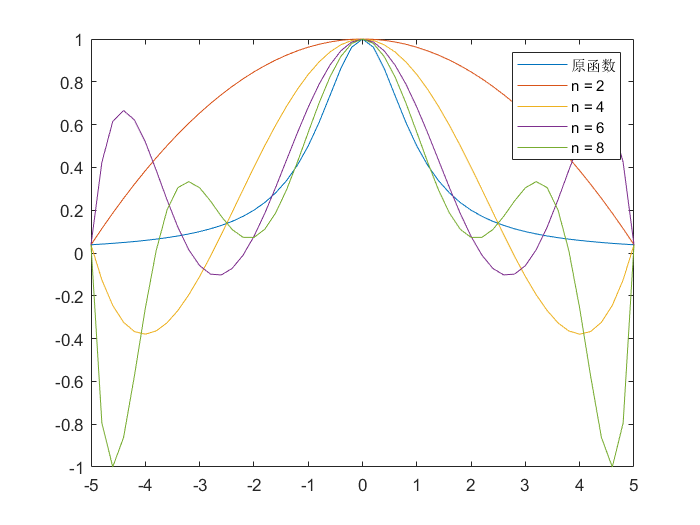
\includegraphics[width=0.5\linewidth]{pic/B.png}
      \caption{Problem B}
    \end{figure}
  \subsection*{} 
    Problem C: test Newton Formula on $\frac{1}{1+25x^2}$ with zeros of Chebyshev polynomials.\\
    n = 5: $0.223856-0.00988929x-0.440012x^{2}+0.0170526x^{3}+0.281243x^{4}$\\
    n = 10: $0.891171+0.797828x-9.16049x^{2}-11.907x^{3}+36.9173x^{4}+51.1959x^{5}-59.7865x^{6}-82.7646x^{7}+32.8302x^{8}+44.604x^{9}$\\
    n = 15: $0.933743+0.285196x-12.6229x^{2}-5.02167x^{3}+88.7539x^{4}+30.6535x^{5}-339.69x^{6}-85.3192x^{7}+730.112x^{8}+119.813x^{9}-877.832x^{10}-83.0762x^{11}+550.437x^{12}+22.6691x^{13}-140.06x^{14}$\\
    n = 20: $0.993612-0.0651879x-22.3507x^{2}+10.7149x^{3}+350.81x^{4}-416.825x^{5}-2998.46x^{6}+5582.53x^{7}+12399.9x^{8}-33851.2x^{9}-18066.4x^{10}+101668x^{11}-24173.6x^{12}-150682x^{13}+107100x^{14}+94115.2x^{15}-117359x^{16}-2625.43x^{17}+42793.2x^{18}-13826.6x^{19}$\\
      \begin{figure}[h]
        \centering
        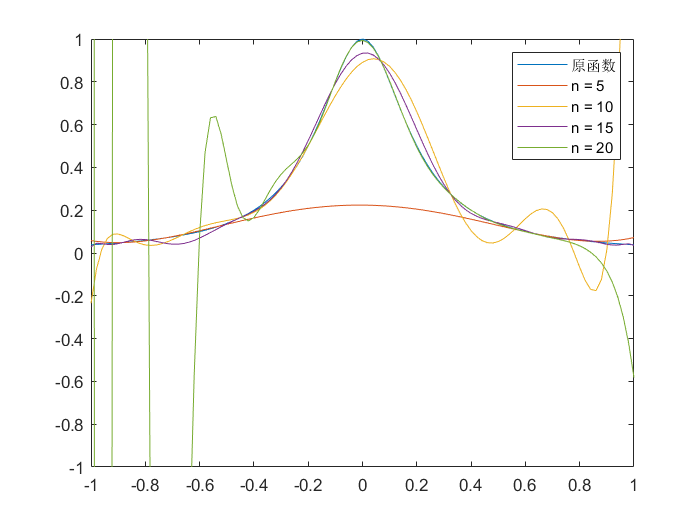
\includegraphics[width=0.5\linewidth]{pic/C.png}
        \caption{Problem C}
      \end{figure}
  \subsection*{} 
    Problem D: Hermite Algorithm on the distance and speed.\\
    polynomial: $75x+7.16191x^{2}-10.0953x^{3}+5.50812x^{4}-1.5383x^{5}+0.243041x^{6}-0.0218757x^{7}+0.00104059x^{8}-2.02236e-005x^{9}$\\
    \begin{figure}[h]
      \begin{minipage}[t]{0.5\linewidth}
      \centering
      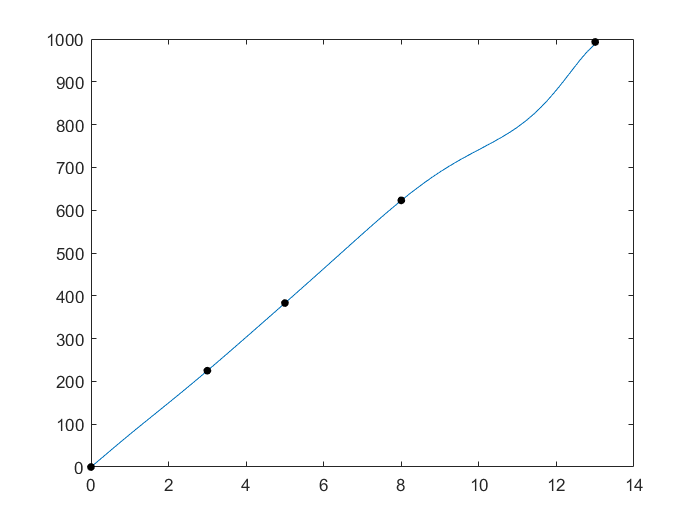
\includegraphics[width=2.2in]{pic/D_1.png}
      \caption{D1}
      \label{fig:side:a}
      \end{minipage}%
      \begin{minipage}[t]{0.5\linewidth}
      \centering
      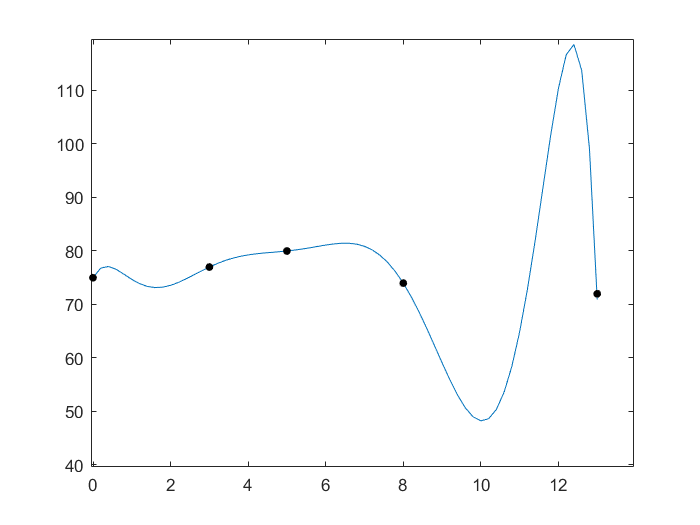
\includegraphics[width=2.2in]{pic/D_2.png}
      \caption{D2}
      \label{fig:side:b}
      \end{minipage}
    \end{figure}
    (a) we can evaluate the position when $t = 10$s: $p(10) = 742.503$ feet.\\
    (b) Obvious from D2 we can see the car has exceeds the speed limit.
  \subsection*{}
    Problem E: approximate the average weight curve for each sample.\\
    sp1:$6.67-43.0127x+16.2855x^{2}-2.11512x^{3}+0.128281x^{4}-0.00371557x^{5}+4.1477e-005x^{6}$\\
    sp2:$6.67-5.85018x+2.98227x^{2}-0.424283x^{3}+0.0265858x^{4}-0.000777473x^{5}+8.6768e-006x^{6}$\\
    It's a bit of odd to see the curve of sp1 has grown to $\bf{negative}$ in some period. 
    Anyway, both two curve shows they grow rapidly when the time has past day 30. 
    \begin{figure}[h]
      \begin{minipage}[t]{0.5\linewidth}
      \centering
      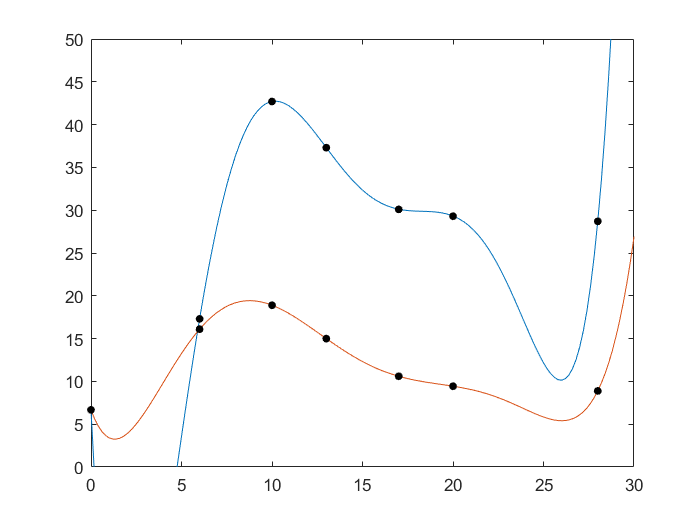
\includegraphics[width=2.2in]{pic/E.png}
      \caption{30days}
      \label{fig:side:a}
      \end{minipage}%
      \begin{minipage}[t]{0.5\linewidth}
      \centering
      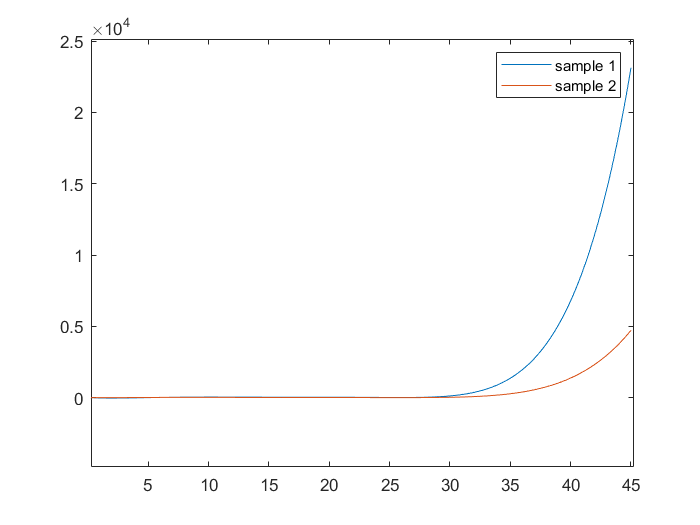
\includegraphics[width=2.2in]{pic/E_1.png}
      \caption{45days}
      \label{fig:side:b}
      \end{minipage}
    \end{figure}
    In day 45, they are in huge numbers. It seems that there's no worry for them to die.
\end{document}
